\documentclass[10pt,a4paper]{article}
\usepackage[a4paper,margin=17mm,top=16mm,bottom=18mm]{geometry}
\usepackage{fontspec,xcolor,graphicx,tabularx,enumitem,hyperref,xurl,fancyhdr,titlesec,needspace,microtype}
\usepackage[english]{babel}
\setlength{\emergencystretch}{2em}
\setmainfont{Lato}\setsansfont{Lato}\renewcommand{\familydefault}{\sfdefault}
\definecolor{Ink}{HTML}{19373F}\definecolor{Teal}{HTML}{176678}\definecolor{Muted}{HTML}{4C636B}\definecolor{Rust}{HTML}{A85731}\definecolor{Rule}{HTML}{D3DFDF}
\hypersetup{colorlinks=true,urlcolor=Teal,linkcolor=Teal,pdfauthor={Dr. Chilperic Armel Foko Kuate},pdftitle={Curriculum Vitae — Dr. Chilperic Armel Foko Kuate}}
\setlength{\parindent}{0pt}\setlength{\parskip}{3pt}\linespread{1.06}\color{Ink}
\setlist[itemize]{leftmargin=1.25em,itemsep=2pt,topsep=3pt,parsep=0pt,label={\color{Rust}\small\textbullet}}
\pagestyle{fancy}\fancyhf{}\renewcommand{\headrulewidth}{0pt}\renewcommand{\footrulewidth}{.4pt}\fancyfoot[L]{\scriptsize\color{Muted}Dr. Chilperic Armel Foko Kuate}\fancyfoot[C]{\scriptsize\color{Muted}Last updated: 4 October 2026}\fancyfoot[R]{\scriptsize\color{Teal}\thepage}
\titleformat{\section}{\large\bfseries\color{Teal}}{}{0pt}{}[\vspace{2pt}{\color{Rule}\titlerule}]\titlespacing*{\section}{0pt}{10pt}{5pt}
\newcommand{\role}[3]{\Needspace{5\baselineskip}{\bfseries #1}\hfill{\small\bfseries\color{Teal}#2}\par{\small\color{Muted}#3}\par}
\newcommand{\degree}[3]{\Needspace{3\baselineskip}{\bfseries #1}\hfill{\small\bfseries\color{Teal}#2}\par{\small\color{Muted}#3}\par\vspace{2pt}}
\newcommand{\project}[2]{\Needspace{4\baselineskip}{\bfseries #1}\par #2\par\vspace{3pt}}
\newcommand{\continued}[1]{{\small\bfseries\color{Teal}DR. CHILPERIC ARMEL FOKO KUATE}\hfill{\small\color{Muted}#1}\par\vspace{5pt}}
\newcommand{\headline}[2]{%
\noindent\begin{minipage}[t]{\dimexpr\linewidth-35mm\relax}
\vspace{0pt}{\small\bfseries\color{Rust}#1}\par\vspace{5pt}
{\fontsize{27}{29}\selectfont\bfseries Dr. Chilperic Armel\\Foko Kuate}\par
\end{minipage}\hfill\begin{minipage}[t]{28mm}
\vspace{0pt}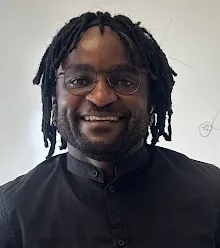
\includegraphics[width=28mm]{profile_photo.png}
\end{minipage}\par\vspace{7pt}
{\large\color{Teal}#2}\par\vspace{9pt}
{\small Düsseldorf, Germany\quad\textbar\quad\href{mailto:chilpericarmel@gmail.com}{chilpericarmel@gmail.com}}\par
{\small\href{https://chilperic.github.io}{Research website}\quad\textbar\quad\href{https://github.com/chilperic}{GitHub}\quad\textbar\quad\href{https://orcid.org/0000-0002-0140-7588}{ORCID: 0000-0002-0140-7588}}\par\vspace{7pt}
{\color{Rust}\rule{23mm}{1.5pt}}{\color{Rule}\rule{\dimexpr\linewidth-23mm}{.5pt}}\par}

\begin{document}
\headline{INDUSTRY CV · COMPUTATIONAL SCIENCE}{Multiscale modelling · Scientific software · Data analysis}
\section{Profile}
Computational scientist with a PhD in quantitative and theoretical biology and research experience in mechanistic modelling, nonlinear dynamics and scientific software. I develop mathematical models and computational workflows that connect assumptions, simulation, observations and interpretation. Target roles: computational scientist, modelling scientist and research software developer in research-intensive teams.
\section{Capabilities}
\begin{tabularx}{\linewidth}{@{}p{35mm}X@{}}
\textbf{Model \& compute} & ODE/DAE systems, enzyme kinetics, stochastic and population models, steady-state and stability analysis.\\[5pt]
\textbf{Analyse \& infer} & Parameter fitting, sensitivity, uncertainty, constrained and derivative-free optimisation; statistical data analysis.\\[5pt]
\textbf{Build \& reproduce} & Python, NumPy/SciPy, SALib, CasADi/IPOPT, CMA-ES; Git, Linux, Jupyter, testing and documentation. Julia, R and MATLAB experience; JavaScript scientific interfaces.
\end{tabularx}
\section{Experience}
\role{Researcher · Computational Cell Biology}{Oct 2026–present}{Heinrich Heine University Düsseldorf · CCB}
Resumed a research appointment on 1 October 2026, continuing computational-biology and mechanistic-modelling work.
\role{Independent research \& FokoLab development}{Nov 2025–Sep 2026}{Düsseldorf, Germany}
Built browser-based scientific tools and maintained modelling repositories; continued research writing and AI/ML training.
\role{Postdoctoral researcher}{Nov 2022–Oct 2025}{CEPLAS / CCB, Heinrich Heine University Düsseldorf}
\begin{itemize}
\item Integrated biochemical, thermal and hydraulic processes in plant-adaptation models; explored environmental response and physiological trade-offs.
\item Developed simulation, optimisation, parameter-exploration and sensitivity workflows, with student supervision and interdisciplinary collaboration.
\end{itemize}
\role{Doctoral researcher · PoLiMeR ITN}{Aug 2019–Aug 2022}{Quantitative and Theoretical Biology, Heinrich Heine University Düsseldorf}
\begin{itemize}
\item Developed kinetic models of hepatic fatty-acid metabolism and synthesis; analysed equilibria, stability and parameter-dependent switching.
\item Contributed to publications on enzyme-kinetic modelling and differentiable constraint-based metabolic models.
\end{itemize}
\newpage\continued{Selected work \& qualifications}
\role{Research fellow}{Nov 2017–Mar 2019}{AIMS · Cameroon and Rwanda}
Stochastic and deterministic T-cell modelling; scientific teaching and computational methods.
\section{Selected technical work}
\project{FokoLab · scientific application}{Connected laboratories for simulation, optimisation, sensitivity, fitting, statistics and mechanistic visualisation. Structured custom models, source attribution, saved experiments and exportable results.\\\href{https://chilperic.github.io/chilperic_ode_solver/site/index.html}{Website} · \href{https://github.com/chilperic/chilperic_ode_solver}{Repository}}
\project{Plant–environment modelling}{A biochemical–thermal–hydraulic framework for photosynthetic adaptation, implemented as reproducible computational experiments. Collaboration includes student research and experimental partners.\\\href{https://github.com/chilperic/photosynthesis-climate-adaptation-model}{Source}}
\project{Metabolic and cell-population models}{Fatty-acid kinetics, nonlinear metabolic behaviour, branching populations and division-tracking models; mathematical formulation paired with numerical analysis.\\\href{https://github.com/chilperic}{Research repositories}}
\section{Education}
\degree{PhD · Quantitative and Theoretical Biology}{2019–2023}{Heinrich Heine University Düsseldorf, Germany. Completed 7 March 2023.}
{\small Dissertation: \textit{Dynamic computational modeling of fatty acid de novo synthesis in the liver and qualitative analysis of fatty acid metabolism.} Supervision: Oliver Ebenhöh; co-supervision and collaboration: Adélaïde Raguin.}\par\vspace{4pt}
\degree{MSc · Mathematics and Fundamental Applications}{2017–2019}{Modelling specialisation · University of Yaoundé I, Cameroon.}
\degree{MSc · Mathematical Sciences}{2015–2016}{AIMS Ghana / University of Cape Coast, Ghana.}
\degree{BSc · Mathematics}{2009–2012}{University of Douala, Cameroon.}
\degree{Baccalauréat}{2009}{Collège La Confiance, Bafoussam, Cameroon.}

\section{Selected publications}
{\small Foko Kuate, Ebenhöh, Bakker \& Raguin (2023). Enzyme-kinetic data for animal fatty-acid synthesis. \textit{Bioscience Reports}. \href{https://doi.org/10.1042/BSR20222496}{\nolinkurl{10.1042/BSR20222496}}.\\[4pt]
Wilken et al., including Foko Kuate (2022). Differentiable constraint-based metabolic models. \textit{Metabolic Engineering} 74, 72–82. \href{https://doi.org/10.1016/j.ymben.2022.09.002}{\nolinkurl{10.1016/j.ymben.2022.09.002}}.}
\section{Teaching, languages \& development}
Supervision of two MSc and two BSc projects; 200+ teaching/tutorial hours. French: native; English: proficient; German: B1/B1+, B2 study ongoing. AI engineering and machine-learning training complement established mechanistic-modelling expertise.

\end{document}
